%%%%%%%%%%%%%%%%%%%%%%%%%%%%%%%%%%%%%%%%%%%%%%%%%%

\chapter{Temas avanzados}

%%%%%%%%%%%%%%%%%%%%%%%%%%%%%%%%%%%%%%%%%%%%%%%%%%

Este capítulo nace de la necesidad de recojer todos los argumentos no
necesariamente ligados al uso de Matlab. La mayoría de ellos están
relacionados con la programación general o en cálculo numérico, sin
embargo son de gran utilidad para escribir buenos programas. La teoría
que contiene este capítulo es de un nivel mucho más elevado al resto,
estais avisados; esto no significa que todo esté explicado del modo
más sencillo posible.

\section{Aumentar la calidad del código escrito en Matlab}

Que el código funcione no suele ser suficiente. Debemos intentar en
cualquier caso escribir código de calidad, debemos convertir en
hábitos ciertas prácticas de programación orientadas a hacer más fácil
el uso de las funciones y los scripts. No todo termina en escribir una
pequeña ayuda en cada función. Hay estrategias muy útiles para
aumentar significativamente la potencia del código escrito sin
necesidad de aumentar el esfuerzo. Debemos entender que si Matlab es
una plataforma de desarrollo rápido de aplicaciones dispondrá de
funciones para escribir código de un modo más eficiente.

\subsection{Vectorizar, la clave para aumentar la velocidad}

Hay muchas maneras de asignar un argumento a una variable. Cuando se
crearon los ordenadores y empezaron a surgir los lenguajes de
programación casi todos los procesos eran escalares. Todo estaba
gobernado por operaciones lógicas que operaban unidades muy pequeñas
de memoria.  A medida que los ordenadores iban creciendo en potencia y
versatilidad se empezó a pensar en una manera más eficiente de
calcular. Uno de los conceptos era la vectorización.\footnote{ Un
  nombre propio en la arquitectura de ordenadores es Seymour Cray, su
  biografía está íntimamente ligada al los ordenadores vectoriales.
  Su influencia es tremenda en el campo de la computación a gran
  escala. }

Se dice que una operación es escalar cuando se hace elemento a
elemento.  Una suma escalar de dos vectores es tomar los elementos de
cada uno de ellos, sumarlos y asignar el resultado a un tercer vector.
Una operación es vectorial cuando se hace por bloques mayores en la
memoria.  Una suma vectorial de dos vectores sería tomar partes del
los vectores o los vectores enteros y sumarlos de golpe.

Los compiladores modernos son capaces de vectorizar automáticamente.
Advierten que dos bucles pueden combinarse perfectamente y realizan la
operación por bloques ahorrando memoria y tiempo de cálculo. Como
Matlab es un programa secuencial carece de esta capacidad de
optimización.  Si nosotros le pedimos un bucle con operaciones
escalares lo va a realizar sin ningún tipo de optimización. Si en
cambio asignamos operamos las matrices mediante la notación matricial
y las submatrices Matlab sí va a ser capaz de vectorizar la operación.

En la sección \ref{sub:El-truco-m=E1s} explicaremos la importancia que
todas estas consideraciones tienen sobre la velocidad de ejecución.

\subsubsection{\label{sub:El-truco-m=E1s}El truco más importante de la
  programación en Matlab}

El truco más importante para que nuestros scripts tengan una velocidad
aceptable es evitar los bucles con contador. Es la estructura más
lenta que existe en el lenguaje. El siguiente ejemplo nos ayudará a
entenderlo perfectamente. Crearemos dos matrices de números aleatorios
y las sumaremos creando una tercera matriz. Primero lo haremos
mediante un bucle que sume con dos índices y luego utilizando el
operador suma elemento a elemento. Utilizaremos la función
\texttt{rand} para crear las matrices y la pareja \texttt{tic} y
\texttt{toc} para calcular el tiempo de cálculo.

\begin{verbatim}
>> a=rand(66); #matriz de 66 x 66
>> b=rand(66);
>> tic;for i=1:66;for j=1:66;c(i,j)=a(i,j)+b(i,j);end;end;toc
ans = 0.17925
>> tic;c=a.+b;toc
ans = 0.00058100
\end{verbatim}
Donde el número que obtenemos como resultado es el tiempo transcurrido
entre la llamada de \texttt{tic} y la de \texttt{toc}. La diferencia
entre los dos métodos es de%
\footnote{El ordenador con el que han sido efectuadas las pruebas es
  un Athlon XP 2600+ (1.920 GHz, bogomips=3301.37) con 512 Mb de RAM a
  400 MHz y Octave 2.1.72. Matlab es ligeramente más rápido con el
  manejo de bucles aunque de ningún modo se acerca a la velocidad de
  los operadores matriciales. Con la optimización máxima Matlab y
  Octave tienen resultados equivalentes. Las pruebas se han efectuado
  diez veces y se da el tiempo medio de la muestra.%
}:

\begin{verbatim}
>> 0.17925/0.00058500
ans = 306.41
\end{verbatim}
Utilizar los operadores matriciales y las submatrices generará código
del orden de 100 veces más rápido. Para una EDP esto es la diferencia
entre un rato de espera y una semana de cálculos, sólo un contador mal
puesto puede acabar con un código globalmente bien escrito.

La lentitud de los bucles llega hasta límites insospechados.
Supongamos que queremos multiplicar todas las filas de una matriz por
un escalar distinto. En un alarde decidimos convertir la serie de
números en un vector y utilizar un bucle contador para operar la
matriz por filas del siguiente modo:

\begin{verbatim}
>> a=1:66;
>> b=rand(66);
>> tic;for i=1:66;c(i,:)=a(i)*b(i,:);end;toc
ans = 0.0032920
\end{verbatim}
Para eliminar este bucle tenemos que convertir la secuencia de números
en una matriz de $66\times66$ y luego multiplicarla por una matriz.
Qué sorpresa nos llevamos cuando observamos que el tiempo de proceso
es menor:

\begin{verbatim}
>> tic;c=a'*ones(1,66).*b;toc
ans = 0.00067000
\end{verbatim}
Eliminando un bucle que parecía completamente justificado acabamos de
reducir el tiempo de proceso a la décima parte.

A partir de ahora nos lo pensaremos dos veces antes de escribir la
palabra \texttt{for}. Si nos acostumbramos pensar con submatrices nos
ahorraremos tiempo de cálculo y la engorrosa tarea de migrar código a
Fortran inútilmente.

\subsubsection{¿Por qué son tan lentos los bucles?}

Lo que hace que los bucles sean tan lentos no es únicamente la
ausencia de vectorización en el cálculo.  Los bucles escalares son muy
rápidos sea cual sea la arquitectura y el lenguaje de programación.
Si analizamos con un poco más de precisión el código de los ejemplos
anteriores observamos que no sólo se están multiplicando dos matrices
o dos escalares, además se está reservando la memoria correspondiente
al resultado.

Imaginemos que queremos sumar dos vectores y asignar el resultado a un
tercero y que para ello utilicemos un bucle.  Primero tomaremos el los
primeros índices de cada vector y los situaremos en una posición de
memoria nueva.  Esto sucederá a cada paso con lo que cada iteración
implicará una operación de reserva de memoria al final de un vector.

Cada vez que ampliamos un vector \emph{llenando} una posición vacía
Matlab debe comprobar que el elemento no existe, ampliar la memoria
reservada al vector para poder situar el nuevo elemento donde debe y
rellenar el resto con ceros y finalmente almacenar los datos del nuevo
vector.

Cuando sumamos dos vectores escalarmente el ciclo de
verificación-reserva -asignación-cierre se realiza una sola vez.
Podemos concluir entonces que la operación de ampliación de una matriz
en Matlab es especialmente lenta.  Aunque no estemos obligados a
declarar las variables antes de inicializarlas es siempre una buena
práctica comprobar que cada matriz se defina entera o mediante bloques
lo suficientemente grandes.

Este comportamiento está ligado al funcionamiento de los arrays en C;
un buen texto para comprenderlo mejor es \cite{Numerical} donde
encontraremos un capítulo inicial sobre qué es verdaderamente un array
y qué relación tiene con un puntero.

Como curiosidad diremos que mientras las operaciones de reserva y
liberación de memoria son bastante lentas, las operaciones de
manipulación de forma como la función \texttt{reshape} son
especialmente rápidas.  No debemos tener miedo a cambiar la forma de
las matrices según nuestras necesidados pensando que estamos
sacrificando tiempo de ejecución.

\subsection{Control de las variables de entrada y salida en
  funciones.(+)}

La necesidad de pasar una cantidad fija de argumentos a una función en
forma de variables no es una limitación para Matlab. Uno de los puntos
débiles de la definición de las cabeceras de las funciones es que no
pueden definirse, tal como lo hacen otros lenguajes de programación,
valores por defecto para las variables de entrada. Matlab cuenta con
la siguiente serie de funciones dedicadas a manipular las variables de
entrada y salida de las funciones:

\begin{description}
\item [nargin\index{nargin}]Da el número de argumentos con el que se
  ha llamado una función
\item [nargoun\index{nargoun}]Retorna el número de argumentos de
  salida de una función
\item [varargin\index{varargin}]Permite que las funciones admitan
  cualquier combinación de argumentos de entrada.
\item [varargout\index{varargout}]Permite que las funciones adimitan
  cualquier combinación de argumentos de salida.
\item [inputname\index{inputname}]Retorna el nombre de la variable que
  se ha pasado como argumento de entrada en una función.
\end{description}
Estas funciones son una ayuda esencial cuando escribimos funciones muy
polivalentes. Los métodos \texttt{nargin} y \texttt{nargout} sirven
para que las funciones se comporten de un modo distinto según la
cantidad de argumentos que reciban, \texttt{varargin} y
\texttt{varargout} hacen que no tengamos que preocuparnos de escribir
largas cabeceras de funciones cuando estas reciben muchos argumentos,
es como si recibiera una variable tipo celda de un modo automático.


\subsection{Comunicación entre el entorno de ejecución global y el
  entorno de la función}

En el léxico utilizado por Matlab se habla de dos entornos de
ejecución o \emph{workspaces}. Existen sólo dos workspaces en los que
habitan varibles inicialmente independientes. El modo usual de
comunicar los dos entornos es mediante variables globales, una vez
definimos una variable como global en todos los \emph{workspace} la
hacemos visible para todas las unidades de programa. Matlab define dos
\emph{workspace}, base y caller. Base es el nombre del entorno de
ejecución principal; sería el intérprete en una sesión interactiva.
Caller es la función que se esté activa en algún momento de la
ejecución. Los dos métodos siguientes son interfaces entre las
variables en base y las variables en caller.

\begin{description}
\item [evalin\index{evalin}]Evalua una variable o una expresión en
  cualquier entorno.
\end{description}
Por ejemplo, vamos a crear una función que intente capturar una
variable del entorno de ejecución principal en una función. Para ello
escribiremos la siguiente función:

\begin{verbatim}
function out=testfunc()
  out=evalin('base','dummy');
\end{verbatim}
Ahora en una sesión del intérprete definiremos la variable
\texttt{var} y veremos cómo queda capturada por la sentencia
\texttt{evalin} sin que aparezca en la cabecera:

\begin{verbatim}
>> testfunc()
error: `dummy' undefined near line 23 column 1
error: evaluating assignment expression near line 2, column 4
error: called from `testfunc'
\end{verbatim}
Nos ha dado un error porque aún no hemos definido la variable
\texttt{dummy} en el entorno base. Si ahora definimos la variable y
llamamos la función:

\begin{verbatim}
>> dummy='hola'
>> testfunc()
ans = hola
\end{verbatim}
Acabamos de comuncar de un modo bastante elegante los dos entornos de
ejecución. Los programadores experimentados están acostumbrados a
lidiar con los punteros. nos podemos imaginar esta función como una
manera razonable de emular el comportamiento de un puntero%
\footnote{Un puntero es un tipo especial de variable cuya misión es
  {}``apuntar'' a una dirección de memoria, normalmente expresada por
  otra variable.  El puntero no es una variable convencional, es
  filosóficamente algo distinto. el contenido de una variable sólo
  podemos cambiarlo nosotros, en cambio el valor al que apunte el
  puntero puede cambiar si así lo exige la ejecución. El concepto de
  un puntero es abstracto y requiere comprender qué es una posición en
  la memoria física de un ordenador.  Es un concepto interesante y
  requiere comprenderlo.%
} y así añadir algo de potencia a nuestros algoritmos. No será
literalmente un puntero porque en vez de apuntar una posición de
memoria apuntará a una variable pero como es la manera normal de
definir los punteros podemos hacer que se comporte del mismo modo. Por
ejemplo, en el caso anterior hemos definido una función que extrae el
valor \texttt{out} que {}``apunta'' al valor contenido en la variable
\texttt{dummy}.  ¿Qué sucede si cambiamos la variable \texttt{dummy}?
Pues que en tiempo de ejecución la variable \texttt{out} cambiará
inmediatamente de valor:

\begin{verbatim}
>> dummy='adios'
dummy = adios
>> testfunc()
ans = adios
\end{verbatim}
Vemos que esto no es exactamente una asignación de una misma posición
de memoria pero la ejecución emula el mismo comportamiento, es como
hacer un \texttt{out==dummy} implícito.

\begin{description}

\item [assignin\index{assignin}]Asigna un valor dado a una variable de
  cualquier entorno de ejecución.
\end{description}

Estas dos funciones es el método recomendado para establecer una
comunicación entre el entorno de ejecución de las funciones y el
entorno principal.  Se sugiere sacrificar el uso de las variables
globales en favor de la asignación y la evaluación entre workspaces.
Sin embargo es una sutileza sujeta al estilo de programación.
Personalmente encuentro las variables globales mucho más intuitivas.


% \subsection{La función \texttt{clear}}

% Más adelante en este capítulo, en la sección \ref{sec:comunica-c-fort}
% y por si aún es ajeno a nosotros este concepto, hablaremos de la
% llamada por valor y la llamada por referencia.  Matlab, como C, llama
% por valor.  Esta característica unida a que podemos iniciar variables
% sin declararlas previamente hace que estemos acumulando memoria en
% uso.  Se llama pérdida de memoria, \emph{memory leak} al defecto que
% se presenta cuando una variable inútil no es destruida y la memoria
% que reserva liberada.

% Algunos lenguajes disponen de un recolector automático de basura pero
% no es el caso de Matlab.  Si creamos una función que utiliza variables
% internas \textbf{Matlab no liberará la memoria que hayan utilizado}
% cuando termine su ejecución.  Si esta función reserva una gran
% cantidad de memoria es muy importante que nos acordemos de utilizar la
% función \texttt{clear} para liberar la memoria utilizada. Incluso
% Fortran, sin recolector de basura y que pasa los argumentos por
% referencia, no tolera estos errores puesto que manda la memoria
% reservada en las subrutinas a un stack o un heap; en el caso de
% desbordarlo da un error en tiempo de ejecución.  Las variables
% verdaderamente grandes requieren una reserva de memoria estática.

% En la mayoría de los programas esto no será necesario, hay que
% trabajar con matrices verdaderamente grandes para ocupar una parte
% significativa de la memoria de un ordenador moderno.  Pero es siempre
% una práctica muy higiénica liberar la memoria al final de cada
% función.  Al igual que en Fortran, la responsabilidad de que un
% programa no tenga pérdidas de memoria recae en el programador, no en
% el lenguaje o sus herramientas.

\section{Array Masking(+)}

Cuando necesitamos controlar el flujo de ejecución de un programa y este
flujo necesita ciertas condiciones lógicas solemos utilizar una 
estructura condicional (\texttt{if}).  Cuando dichas condiciones lógicas
adquieren un alto grado de complejidad, con más de seis o siete opciones
que pueden ser complementarias entre ellas, la implementación de la
estructura suele ser harto complicada.

En programación suelen evitarse este tipo de estructuras, son lentas,
difíciles de programar, difíciles de entender y propensas a generar
errores en tiempo de ejecución que cuesta bastante resolver. En otros
lenguajes de programación los defectos de forma suelen ser los más
importantes pero ya hemos aprendido que en Matlab es una buena práctica
programar con la velocidad en mente.

Una solución especialmente eficiente es ver que los grupos de números
binarios son un conjunto no intersectado en los que las operaciones de
adición, sustracción y combinación lógicas son triviales. Esto sirve para
constuir encima de cada matriz una {}``máscara lógica'' que permite
asignar una etiqueta a cada elemento de la matriz.

\section{Introducción al debbugging}

La traducción de la palabra debugging es {}``quitar los bichos''.  Un
bug o bicho es un error en el código, sus efectos pueden ser evidentes
o sutiles y la tarea de encontrarlos es mucho más complicada que
eliminarlos.  Los debuggers son programas especiales para esta tarea
de uso en lenguajes compilados. Lo que hacen es ejecutar los procesos
paso a paso para conocer su funcionamiento de un modo más interactivo.
Matlab ya es en sí mismo interactivo pero algunas herramientas del
debugging clásico serán útiles en programas muy grandes.

El debugging se basa en los \emph{breakpoints} que no son más que
puntos en los que podemos detener la ejecución del programa para
analizar su estado actual. La posición de los breakpoints es más una
labor de experiencia que una ley tanto en los lenguajes compilados
como interactivos. Solemos poner uno antes de llamar una función y
unos cuantos antes de que aparezca el error.

El editor de Matlab es además el interfaz para el debugger. Podremos
poner y quitar los breakpoints con el ratón y recuperar el control del
proceso con la consola. Pero cuando uno se siente cómodo con el
debugging prefiere realizar todo el proceso manualmente mediante las
funciones propias. Estas funciones son casi las mismas en Matlab y
Octave.

\begin{description}
\item [keyboard]Esta palabra clave no es parte del debugging en
  sentido estricto pero puede ser muy útil para resolver errores del
  código.  Si introducimos esta función en un programa pararemos su
  ejecución y pasaremos a tener el control en el punto de ejecución
  donde nos encontremos. Se abrirá un intérprete mediante el cual
  accederemos al estado actual del programa para poder acceder a las
  variables de modo interactivo. Una vez salgamos del intérprete
  continuaremos la ejecución conservando los cambios que hayamos
  introducido. Este es el modo más sencillo de hacer debugging en
  scripts porque las funciones para debugging clásicas sólo operan
  dentro de funciones.
\item [{echo}] \index{echo}Traducido eco.  Controla si los comandos en
  archivos aparecen o no en pantalla. Esta sentencia sólo tiene efecto
  dentro de un archivo o de una función.  Normalmente los comandos
  ejecutables de funciones y scripts no aparecen en pantalla, sólo
  aparece su resultado si no hemos puesto un punto y coma al final de
  la línea. Con \texttt{echo on} los comandos de los scripts se
  escriben como si los hubieramos introducido a través
  del intérprete.\\
  \\
  \begin{minipage}[c]{1\linewidth}%
    \texttt{on} Activa el eco en los scripts

    \texttt{off} Desactiva el eco en los scripts

    {\texttt{on all}} Activa el eco en scripts y funciones

    {\texttt{off all}} Desactiva el eco en scripts y
    funciones\end{minipage}%

\item [type\index{type}]Saca por pantalla el texto correspondiente a
  cualquier función que esté en el árbol de directorios dentro de un
  archivo \texttt{.m}.  Es útil cuando disponemos de una colección
  propia de funciones bastante extensa y preferimos no abrir el
  archivo con el editor.
\end{description}
Como ejemplo del uso de las funciones de debugging utilizaremos el
script \texttt{polyadd.m} que implementa la suma de dos polinomios.
Las rutinas básicas para el debugging de funciones son:

\begin{description}
\item [dbtype\index{dbtype}]Muestra la función con los números de
  línea para facilitar la inclusión de breakpoints
\end{description}
Para usarlo con nuestra función sería

  \begin{verbatim}
>> dbtype polyadd
1       function poly=polyadd(poly1,poly2)
2         if (nargin != 2)
3           usage('polyadd(poly1,poly2)')
4         end
5         if (is_vector(poly1) && is_vector(poly2))
6           if length(poly1)<length(poly2)
7             short=poly1;
8             long=poly2;
9           else
10            short=poly2;
11            long=poly1;
12          end
13          diff=length(long)-length(short);
14          if diff>0
15            poly=[zeros(1,diff),short]+long;
16          else
17            poly=long+short;
18          end
19        else
20          error('both arguments must be polynomials')
21        end
\end{verbatim}
Ahora queremos colocar dos breakpoints, uno en la línea 14 y otro en
la línea 16. Para ello usaremos la siguiente función:

\begin{description}
\item [{dbstop\textsl{(func,line)}}\index{dbstop}]Introduce un
  breakpoint en una función.
\end{description}
\begin{verbatim}
>> dbstop('polyadd','14')
ans = 14
>> dbstop('polyadd','16')
ans = 17
\end{verbatim}
Fijémonos que la función no nos ha dejado poner el breakpoint en la
línea 16 porque no es ejecutable. Para comprobar el estado de la
función:

\begin{description}
\item [dbstatus]Devuelve un vector cuyos elementos son las líneas con
  breakpoints.
\end{description}
\begin{verbatim}
>> dbstatus polyadd
ans =
  14  17
\end{verbatim}
Ahora utilizamos la función del modo usual. La ejecución avanzará
hasta que encuentre un breakpoint, entonces se abrirá una consola que
nos dará el control de la ejecución.

  \begin{verbatim}
>> polyadd([3,2,1,3],[3,2,0])
polyadd: line 14, column 8
diff
debug>
\end{verbatim}
La consola \texttt{debug} es local, es decir, sólo contiene las
variables de la ejecución de la función. Lo más lógico en este punto
es utilizar la función \texttt{who} para saber qué variables han sido
iniciadas:

  \begin{verbatim}
debug> who
*** local user variables:
__nargin__   argn         long         poly1        short
__nargout__  diff         poly         poly2
\end{verbatim}
Aprovechamos para conocer algunas de ellas:

  \begin{verbatim}
debug> long
long =
  3  2  1  3
debug> poly1
poly1 =
  3  2  1  3
debug> poly2
poly2 =
  3  2  0
debug> __nargin__
__nargin__ = 2
\end{verbatim}
\texttt{\_\_nargin\_\_} es el número de argumentos de entrada. Si
salimos de la consola avanzaremos hasta el siguiente breakpoint o
finalizaremos la ejecución. En este caso llegaremos hasta la línea 17.

Para eliminar alguno de los breakpoints:

\begin{description}
\item [{dbclear\textsl{(func,line)}}\index{dbclear}]Elimina el
  breakpoint de la línea solicitada.
\end{description}
\begin{verbatim}
>> dbclear('polyadd','17')
polyadd
symbol_name = polyadd
>> dbstatus polyadd
ans = 14
\end{verbatim}
Hay más comandos para debugging pero estos son los más importantes.


\section{Extender Octave con otros
  lenguajes.\label{sec:Extender-Octave-con}}

\emph{Gran parte de esta sección, sobre todo los ejemplos, se basa en
  el tutorial {}``Dal segno al Coda'' de Paul Thomas. Podeis
  encontrarlo en el Wiki del proyecto Octave.}

Octave está escrito en C++, además es el lenguaje desde el que es más
sencillo extenderlo. Ahora deberíamos preguntarnos cuándo queremos
extender Octave. Si Matlab es un lenguaje de programación completo
deberíamos ser capaces de programar cualquier cosa. El problema es que
programar cualquier cosa no se hace a cualquier precio, los bucles son
un ejemplo de ello. Imaginemos que tenemos un programa que va
demasiado lento, que casi todo el tiempo de proceso se debe a la
evaluación de una función miles de millones de veces y el coste de
implementarla en otro lenguaje no es demasiado grande. La solución a
nuestro problema será escribir la función en C++ o en Fortran y luego
hacer un interfaz para que Octave pueda entenderla.

Para hacerlo antes tendremos que asegurarnos que disponemos de las
cabeceras (headers) de Octave. No se encuentran en algunos paquetes y
puede ser que tengamos que instalarlos a parte. Preparar la
infraestructura es un poco complejo, también necesitaremos un
compilador en el entorno accesible por consola, preferentemente los de
la colección gcc (gcc, g++, g77 y gfortran).

Las cabeceras sirven tanto para escribir pequeñas funciones como para
crear interfaces completos a librerías escritas en C, C++ o Fortran.
\texttt{mkoctfile} es la herramienta básica del desarrollo de Octave,
todos los archivos terminados en \texttt{.oct} han sido creados con
dicha función. Algunas de las librerías utilizadas son FFTW para las
transformadas rápidas de Fourier, ODEPACK para resolver ecuaciones
diferenciales ordinarias, UMFPACK para las matrices sparse y ATLAS
para el cálculo matricial. Los respectivos interfaces son una gran
fuente de información de cómo adecuar Octave a nuestras necesidades.


\subsection{Una advertencia antes de empezar a programar.}

Es posible que cuando probemos alguno de los ejemplos que se expondrán
a continuación recibamos un \emph{segmentation fault} o un resultado
sin ninguna lógica en vez de lo esperado. Muchas veces los programas
no son compilar y listo, los programadores experimentados en C y C++
saben de lo que hablo. Otra de las ventajas de los lenguajes
interpretados es que el intérprete es un binario \emph{standalone}%
\footnote{Este término informático proveniente de la expresión
  \emph{to stand alone} es el adjetivo que recibe un programa que
  despues de ser compilado ya no tiene ninguna dependencia externa;
  puede tenerlas en tiempo de compilación pero no en tiempo de
  ejecución. En un sistema operativo tipo UNIX esto es imposible
  porque todo depende como mínimo de la librería estándar de C.%
}. Octave es un programa que depende de varias librerías
externas, glibc, atlas, readline... Todas estas librerías deben ser
compiladas previamente de tal modo que sean compatibles con el
intérprete de Octave. Es normal que alguna de las dependenicas se
construya con un compilador distinto al que se utilice para Octave.
Normalmente no tendremos ningún problema pero esto no implica que no
se produzcan jamás.

Un ejemplo de ellos es cuando intentamos añadir código externo a
Octave con el programa mkoctfile. Lo que estamos haciendo es compilar
un archivo escrito en C++ con el compilador del sistema que puede ser
distinto al que se utilizó para Octave. Es incluso probable que los
compiladores sean incompatibles como por ejemplo el GCC4 y el intel
C++ compiler. Debemos tener en cuenta que Octave es a partir de ahora
un verdadero entorno de desarrollo, único y monolítico. Si queremos
ponernos a jugar de verdad lo mejor será que compilemos nosotros
mismos Octave con el compilador del sistema. Si somos incapaces de
hacerlo instalaremos el compilador con el que se construyó nuestro
Octave así como las librerías propias de C y C++ sobre las que
funciona.

Si podemos tener problemas con los compiladores de C++ con los de
Fortran debemos prepararnos para sufrir de lo lindo. Octave se compila
con gcc3, sin soporte para Fortran 95. Si queremos utilizar código en
este dialecto tendremos que utilizar gcc4 pero entonces las versiones
de las librerías de C++ serán incompatibles. Disponemos de dos
opciones:

\begin{enumerate}
\item Seguir con gcc3, escribir código en Fortran 77 y compilar con
  g77.
\item Pasarnos a la rama inestable de Octave, compilarla con gcc4 y
  gfortran y rezar para que no rompa nada.
\end{enumerate}
Por suerte estos problemas desaparecerán cuando gcc4 se consolide.


\subsection{Extender Octave con C++}

Una vez tengamos toda la infraestructura preparada podemos acoplar
cualquier función escrita en C++ a Octave. La diferencia entre los
archivos \texttt{.oct} y los \texttt{.mex} de Matlab es que en este
caso contamos con cabeceras que nos permiten manipular directamente
los argumentos de Octave. El header principal es \texttt{oct.h}, en él
se encuentran las definiciones de todos los argumentos necesarios.

Empezaremos con el siguiente archivo de ejemplo que llamaremos
\texttt{eqlorentz.cc}:

\begin{verbatim}
#include <octave/oct.h>
DEFUN_DLD (eqlorentz,args, ,
    "Ecuacion de Lorentz en C++")
    {
    ColumnVector xdot (3);
    ColumnVector x (args(0).vector_value());
    int a=10;
    int b=28;
    double c=8./3;
    xdot(0) = a*(x(1)-x(0));
    xdot(1) = x(0)*(b-x(2))-x(1);
    xdot(2) = x(0)*x(1)-c*x(2);
    
    return octave_value (xdot);
    }
\end{verbatim}
Esta es la función de la ecuación diferencial del atractor de Lorentz:
$$
\begin{array}{l}
  \dot{x}=a(y-x)\\
  \dot{y}=x(b-z)-y\\
  \dot{z}=xy-cz\end{array}\qquad con\qquad 
a=10,\,\, b=28,\,\, c=\frac{8}{3}$$

Encontraremos el script que resuelve el problema en el ejercicio
\ref{sec:Ejercicio ode}.  Tenemos que evaluar la ecuación del atractor
un mínimo de 5000 veces, nos ahorraremos algo de tiempo escribiendo la
función en C++ y convirtiéndola en una función de Octave con:

\begin{verbatim}
bash ~/> mkoctfile eqlorentz.cc
\end{verbatim}

El resultado será un archivo llamado \texttt{eqlorentz.oct} que es
equivalente a cualquier archivo de función:

\begin{verbatim}
>> help eqlorentz
eqlorentz is the dynamically-linked function from the file
/home/guillem/sync/CursoScripting/ejercicios/eqlorentz.oct
Ecuacion de Lorentz en C++
>> eqlorentz([1,1,1],1)
ans =
    0.00000
   26.00000
   -1.66667
\end{verbatim}

Otra posibilidad interesante es la de crear subrutinas optimizadas
para un tipo determinado de hardware. No es lo mismo llamar a una
subrutina que funcionaría en cualquier PC que optimizarla para
utilizar todas las posibilidades de un Xeon o de un Opteron.
\texttt{mkoctfile} no es más que un interface a los compiladores de la
família gcc, podemos pasarle parámetros de compilación para conseguir
una optimización máxima.

\subsubsection{Llamar funciones desde C++}

A medida que nos introduzcamos en la programación de extensiones para
Octave es probable que tengamos la necesidad de tomar funciones como
argumentos.  Un posible ejemplo de ello sería una rutina de integración
de una EDO; sin la función es imposible integrar nada.

Llamar una función desde Octave no es difícil pero tampoco es trivial.
Disponemos del tipo \texttt{octave\_function} que contiene todos
los métodos necesarios, el problema (si es que lo es) es que debe
referirse al argumento como un puntero.  Un \texttt{octave\_function} va a ser
siempre un puntero a una función.  Lo demás es ser un poco congruente
con la definición hecha anteriormente; una función se llama
mediante el método \texttt{do\_multi\_index\_op} que recibe como argumentos
el número de variables de entrada y un \texttt{octave\_value\_list} con
los mismos.  La salida será también un \texttt{octave\_value\_list}.

Ya en octave, para pasar las funciones debemos utilizar un function
handle, una función anónima o la función \texttt{inline}, de otro modo
Octave no sabrá que uno de los argumentos es una función.  Para que
la propia rutina lo compruebe se utilizan los métodos 
\texttt{is\_function\_handle} y \texttt{is\_inline\_function}.

Para ilustrar todo lo anterior utilizaremos el siguiente ejemplo:

\begin{verbatim}
/*testfh.cc*/
# include <octave/oct.h>

DEFUN_DLD(testfh,args, ,
          "testing how C++ can call an octave function")
{
  octave_value_list tmp;
  octave_value_list inval;
  octave_function *input_fcn=0;
  if (args(0).is_function_handle() || args(0).is_inline_function())
    input_fcn = args(0).function_value();
  else
    {
      error("this is not a function handle nor an inline function");
      return octave_value(-1);
    }
  double x = args(1).double_value();
  inval.append(octave_value(x));
  tmp = input_fcn->do_multi_index_op(1,inval);
  return tmp;
}
\end{verbatim}

Esta función recibe un function handle o un inline y un escalar de doble
precisión. Retorna la función evaluada en el punto definido por el escalar.
Para compilarlo haremos:

\begin{verbatim}
bash~/> mkoctfile testfh.cc
\end{verbatim}

Ya dentro de Octave ensayaremos su funcionamiento:

\begin{verbatim}
>> testfh('sin',.123)
error: this is not a function handle nor an inline function
>> testfh(@sin,pi/2)
ans = 1
>> testfh(@(x) sin(x)*exp(x/2),pi/4)
ans = 1.0472
>> testfh(inline('sin(x)*exp(x/2)'),pi/4)
ans = 1.0472
\end{verbatim}

Como vemos es capaz de entender function handles, function handles y
funciones inline.  Esta capacidad abre significativamente el abanico
de posibilidades de octave.  Las funciones escritas en C++ ya no son
algo monolítico, es decir, una subrutina tonta que sólo es capaz de
recibir y devolver valores.  Ahora podemos interactuar con toda
la plataforma de octave, incluso con las funciones pasadas por
cabecera.

\subsection{Extender Octave con Fortran}

Fortran es el lenguaje de cálculo científico por excelencia. Se ha
abandonado paulatinamente durante los últimos años por el hecho de que
no había ningún compilador libre de Fortran 95. Este hueco ha sido
llenado por los compiladores G95 y gfortran%
\footnote{gfortran es un fork del proyecto G95 por desavenencias en el
  desarrollo con su creador. gfortran está dentro de gcc mientras que
  G95 es un proyecto a parte.%
}. Ahora cualquier desarrollador puede programar en Fortran sin
necesidad de aceptar licencias restrictivas sobre su código.

Evidentemente el lenguaje de extensión natural de Octave es C++ pero
disponemos de la cabecera \texttt{f77-fcn} para comunicarnos con
subrutinas escritas en Fortran. Siendo Fortran tan popular en el
ámbito científico es lógico que Octave le de un trato especial.
Desgraciadamente la capacidad de integración de Fortran en Octave es
bastante limitada debido sobre todo a las dificultades de comunicación
entre C y Fortran.  Otros lenguajes interpretados cumplen mucho mejor
la labor de comunicarse con sus primos compilados como Python, Java o
Ruby.


\subsubsection{¿Por qué Fortran?}

Las subrutinas escritas en Fortran no son más rápidas en Octave que
las escritas en C++ sin embargo Fortran tiene otras muchas ventajas.
Fortran es, además de un lenguaje para aplicaciones científicas por
excelencia, el único en el que el uso de memoria es puramente
matricial.  Cuando declaramos un array en Fortran 95 lo hacemos con
rango, no sólo con la cantidad de memoria necesaria. Fortran es
claramente mejor que cualquier otro lenguaje de programación cuando
hay que calcular con variables de gran tamaño. Cuando operamos con
vectores, matrices y tensores a la vez es muy fácil equivocarse en los
índices o {}``pisar'' fuera de la matriz. Fortran reserva memoria de
una manera estricta y no tolera un mal uso de ella.

Otro motivo de peso es la manera radicalmente distinta en la que
Fortran y C tratan los arrays.  Mientras en Fortran el uso de la
memoria está detrás del concepto de array, en C no es más que una
sucesión de posiciones de memoria contiguas.  Cuando uno aprende C sin
ser un experto en ordenadores el concepto de puntero se le hace
tremendamente antinatural; más aún si la experiencia previa es en
Fortran. C es un lenguaje especialmente pequeño, esa es su gran
ventaja; pero no por ello es más simple o genera menos sutilezas.
Veamos por ejemplo los dos programas siguientes en C++.  En ellos se
pretende llamar a la ecuación diferencial de Lorentz y sacar el
resultado por pantalla.

\begin{verbatim}
#include <iostream>
using namespace std;

void lorentz(double t,double *y,double *yp)
{
  const int a=10;
  const int b=28;
  const double c=8./3;
  yp[0]=a*(y[1]-y[0]);
  yp[1]=y[0]*(b-y[2])-y[1];
  yp[2]=y[0]*y[1]-c*y[2];
}

int main(int argc,char *argv[])
{
  double y[3];
  double yp[3];

  y[0]=1.;
  y[1]=1.;
  y[2]=1.;
  lorentz(1.,y,yp);
  int i;
  for (i=0;i<3;i++)
    {
      cout << yp[i] << '\n';
    }
  return 0;
}
\end{verbatim}

La salida por pantalla es la siguiente:
\begin{verbatim}
guillem@desktop:~$ ./a.out
0
26
-1.66667
\end{verbatim}

Que es precisamente el resultado de la ecuación diferencial. Llama la
atención el hecho que en la cabecera no hemos definido ningun array
sino punteros.  En la cabecera de la función las definiciones

\begin{verbatim}
*double
double[3]
double[]
\end{verbatim}
Son equivalentes.

Ahora pensamos que a lo mejor C++ es muy listo y que podemos
ahorrarnos el bucle para obtener el resultado.  Probamos lo siguiente:

\begin{verbatim}
#include <iostream>
using namespace std;

void lorentz(double t,double *y,double *yp)
{
  const int a=10;
  const int b=28;
  const double c=8./3;
  yp[0]=a*(y[1]-y[0]);
  yp[1]=y[0]*(b-y[2])-y[1];
  yp[2]=y[0]*y[1]-c*y[2];
}

int main(int argc,char *argv[])
{
  double y[3];
  double yp[3];

  y[0]=1.;
  y[1]=1.;
  y[2]=1.;
  lorentz(1.,y,yp);
  int i;
  cout << yp << '\n';
  
  return 0;
}
\end{verbatim}

Y al ejecutar el programa:
\begin{verbatim}
0xbfce1360
\end{verbatim}
El programa ha escupido una dirección de memoria.  Para un programador
experimentado en C esto resultará tan obvio como desconcertante para
el resto de los mortales.  La relación entre los arrays y los punteros
es de amor-odio.  Salpica cualquier programa escrito en C o en C++ y
puede llegar a ser una tortura cuando sólo nos interesan los arrays.
Fortran no sólo es más seguro sino que ayuda a programar con pocos
errores tanto en la implementación del algoritmo como en el uso de la
memoria.

Otra ventaja importante es que la biblioteca estándar de Fortran
contiene funciones orientadas al cálculo científico y que la mayoría
de las bibliotecas de cálculo numérico están pensadas para comunicarse
con Fortran y no con C o C++.


\subsubsection{La difícil comunicación entre C y Fortran}
\label{sec:comunica-c-fort}
Fortran y C son lenguajes diametralmente opuestos, sobretodo en el uso
de la memoria. Mientras C permite al usuario jugar con las direcciones
de memoria de un modo transparente, incluso accediendo explícitamente
a los registros; Fortran utiliza la memoria en sentido estricto y
dejando pocas libertades al usuario. La gran diferencia entre ambos es
sin duda las llamadas a funciones y subrutinas, C llama por valor y
Fortran por referencia. ¿Qué significa eso? No olvidemos que Matlab
está escrito en C y Octave en C++, ambos utilizan una infraestructura
equivalente a cualquier programa en C. Para entender bien qué es una
llamada por valor y una llamada por referencia es necesario que
entendamos qué es una dirección de memoria y qué es un puntero.

Los ordenadores tienen tres tipos de memoria: la memoria cache, la
memoria física y la memoria virtual. La más importante de ellas para
un programa es la memoria física y es en la que debemos pensar cuando
programamos. Entrar en más disquisiciones sobre arquitectura de
ordenadores ahora sería inútil. Los programas no son más que procesos
de gestión de memoria; es almacenar algo en un sitio y decir qué hay
que hacer con ello. Si queremos sumar 2 más 2 tendremos que almacenar
un 2 en una posición de memoria, un 2 en otra, pasarlas por un sumador
y luego almacenar el resultado. Los lenguajes de programación de alto
nivel permiten escribir programas sin tener que pensar en todas estas
sutilezas.

Cuando en un código asignamos una variable a un argumento:

\begin{verbatim}
a=2
\end{verbatim}

estamos haciendo dos cosas: primero reservamos el espacio en memoria
necesario para almacenar un 2 y luego le estamos asignando el nombre
de una variable. El nombre está sólidamente unido a la posición de
memoria. Ahora supongamos que queremos referirnos a la variable a.
Podemos hacerlo de dos maneras. La primera es llamar el contenido de
a, es decir, 2. La segunda es referirnos a la variable según la
posición de memoria que ocupa. Llamamos posición de memoria a el punto
de la memoria física en el que se encuentra \emph{realmente} contenida
la variable y se expresa mediante una \emph{dirección de memoria} que
suele ser una cadena de 8 caracteres.

Esto nos permite distinguir entre dos tipos esenciales de variables,
las que contienen un valor y las que apuntan a una determinada
dirección de memoria. Las primeras se llaman variables y las segundas
reciben el nombre de \emph{punteros}. Los programadores experimentados
en C y C++ dominan el concepto de puntero pero los que no lo hayan
oído en su vida lo entenderán mejor con este pequeño programa en C:

\begin{verbatim}
#include <stdio.h>
int a;
int *ptr;
int main(int argc, char *argv[])
{
  a=2;
  ptr =  &a;
  printf("a es %i \n",a);
  printf("la direccion de a es %p \n",ptr);
  printf("el puntero ptr contiene %i \n",*ptr);
  return 0;
}
\end{verbatim}

Primero declaramos una variable de tipo entero y luego un puntero del
mismo tipo, luego le asignamos a la variable el valor de 2 y el
puntero a la posición de memoria de la variable. Imprimimos en
pantalla el resultado para saber qué contiene cada una de ellas y el
resultado es el siguiente:

\begin{verbatim}
a es 2
la direccion de a es 0x403020
el puntero ptr contiene 2
\end{verbatim}

Una vez hemos entendido la diferencia entre una posición de memoria y
el valor que esta contiene daremos el siguiente paso. Supongamos que
acabamos de escribir una función o una subrutina. Esta unidad de
programa necesita argumentos adicionales para funcionar especificados
en su cabecera. Si la función no recibe los argumentos necesarios en
tiempo de ejecución recibiremos un error. Pero acabamos de ver que
para el ordenador es equivalente recibir un valor que la posición de
memoria del bloque que la contiene. En un programa parecido al
anterior definimos la una función suma:

\begin{verbatim}
#include <stdio.h>

int a,b;
int sum(int a,int b)
{ 
  int result;
  result=a+b;
  return result;
}

int main(int argc, char *argv[])
{
  a=2;
  b=3;
  int resultado=sum(a,b);
  printf("la suma de %i y %i es %i \n",a,b,resultado);
  return 0;

}
\end{verbatim}

¿Qué hace C para pasar los valores a la función? C pasa los argumentos
a las funciones por valor. Esto significa que las memoria utilizada
por la función y por el programa principal son independientes. Cuando
pasamos los argumentos a la función suma se copia su valor a las
variables locales sin tocar las globales; la función espera un valor,
no una dirección de memoria; espera un 2, no un 0x748361.

Fortran es diametralmente opuesto a C en este sentido. Todas las
variables de Fortran son en realidad punteros. Fortran no sabe de
valores reales, sólo está interesado en posiciones de memoria. La
identificación entre la memoria y la variable es absoluta. Vamos a
descifrar lo dicho hasta ahora mediante un programa ejemplo:

\begin{verbatim}
program test
integer :: a,b,c
a=2
b=3
call sum(a,b,c)
write(*,*) c
end program test


subroutine sum(arg1,arg2,resultado)
  integer, intent(in) :: arg1,arg2
  integer, intent(out) :: resultado
  resultado=arg1+arg2
end subroutine sum
\end{verbatim}

Cuando llamamos a la subrutina sum no estamos pasando los valores 2 y
3 sino que estamos identificando las posiciones de memoria. Le estamos
diciendo a la subrutina que su arg1 se encuentra en la posición de a y
arg2 en la de b. Por eso tenemos que declarar las variables en las
subrutinas con el atributo intent; estamos operando con las mismas
posiciones de memoria, si nos equivocamos no podemos volver atrás.
Esto se llama pasar los argumentos por \emph{referencia}. Este punto
de vista es mucho menos versatil pero evita el uso de más memoria de
la necesaria. Por eso Fortran es un lenguaje muy indicado para manejar
variables de gran tamaño.

Esto significa que programando en C tendremos que pasar punteros y no
variables a las funciones escritas en Fortran.


\subsubsection{Llamar una función de C desde Fortran o la manera más difícil de sumar 2+2}

Para entender mejor el significado de la llamada por referencia en
Fortran vamos a aprovechar que los archivos objeto creados con el GCC
son independientes del frontend utilizado.  La estrategia es la
siguiente, crearemos una función en C que sume la primera y la segunda
variable y retorne el resultado en la tercera.  El código es el
siguiente:
\begin{verbatim}
void c_function_(int *a,int *b,int *c)
{
  *c=*a+*b;
}
\end{verbatim}
Algunas observaciones importantes:
\begin{enumerate}
\item Las funciones del tipo \texttt{void} son equivalentes a las
  subrutinas en Fortran.
\item El nombre de la función va seguido de una barra baja (trailing
  underscore) para que el nombre de la subrutina generada sea
  compatible con Fortran.  Ignoro el por qué pero de otro modo no
  funciona.
\item Como la función espera una asignación de argumentos por
  referencia espera punteros a las variables.  En la función debemos
  ser consecuentes y utilizar el operador de retorno de referencia
  para hacer la operación.
\end{enumerate}
Compilamos la función con:
\begin{verbatim}
bash$~/> gcc -c c_function.c
\end{verbatim}

Sólo falta crear el programa que implemente la llamada.  Es el
siguente:
\begin{verbatim}
program fortran_c_call

  integer :: a,b,c

  a=2
  b=2

  call c_function(a,b,c)

  write(*,*) c
end program fortran_c_call
\end{verbatim}
Lo compilamos y lo ejecutamos:
\begin{verbatim}
bash$~/> gfortran fortran_c_call.f90 c_function.o
bash$~/> a.out
        4
\end{verbatim}
Esta operación es imposible si el código objeto generado es
incompatible. Por muy extraño que parezca este tipo de
interoperabilidad es típica de un sistema UNIX.  Aunque C y Fortran
puedan parecer a veces agua y aceite no debemos olvidar que los
compiladores de Fortran no son más que programas escritos en C.

\subsubsection{Punteros y arrays}

El tipo esencial de Fortran es el array. Un array es un bloque de
memoria que contiene elementos del mismo tipo. Definimos un array
siempre con el apellido de su tipo; hablamos de array de enteros,
array de reales de doble precisión... En las variantes de Fortran más
recientes los arrays tienen rango. Fortran no trata del mismo modo un
array de rango 2 que uno de rango 3, ordenará los elementos de un modo
distinto para optimizar la lectura y la escritura. Hemos dicho que
todas las variables son en realidad punteros; un array es un puntero
al primer elemento, una sentencia de reserva de la memoria necesaria y
una regla de lectura y escritura. Si intentamos leer un elemento fuera
de los límites del array Fortran nos dará un error en tiempo de
ejecución

C no tiene ningún método para definir arrays, C sólo sabe reservar
memoria. Si intentamos emular el comportamiento de Fortran debemos
tener mucha precaución. Por mucho que intentemos reservar la memoria
justa y no llamar ningún elemento que no exista dentro de la variable
el rango desaparece. Para C estas dos declaraciones:

\begin{verbatim}
array[15];
array[3][5];
\end{verbatim}
son equivalentes. Será muy importante utilizar las cabeceras de Octave
porque nos proporcionarán los tipos necesarios para utilizar
cómodamente matrices y arrays.


\subsubsection{Escritura de \emph{wrappers} para funciones en
  Fortran.}

Aunque este es un conveniente importante no se requieren grandes
conocimientos de C++ para escribir uno. Para escribir un wrapper a la
ecuación diferencial del atractor de Lorentz:

\begin{verbatim}
subroutine eqlorentzfsub(x,xdot)
  real(8),dimension(:),intent(in) :: x
  real(8),dimension(:),intent(out) :: xdot
  real(8) :: a=10d0,b=28d0
  real(8) :: c
  c=8d0/3d0
  xdot(1)= a*(x(2)-x(1))
  xdot(2)= x(1)*(b-x(3)-x(2))
  xdot(3)= x(1)*x(2)-c*x(3)
end subroutine eqlorentzfsub
\end{verbatim}
El wrapper correspondiente para esta función es el siguiente:

\begin{verbatim}
#include <octave/oct.h>
#include "f77-fcn.h"
extern "C" int F77_FUNC (eqlorentzfsub,
                           EQLORENTZFSUB)(double*,double*);
DEFUN_DLD(eqlorentzf,args, ,"xdot=eqlorentz(x)")
{
  octave_value_list retval;
  ColumnVector wargin(args(0).vector_value());
  ColumnVector wargout(3);
  F77_FUNC(eqlorentzfsub,EQLORENTZFSUB)(wargin.fortran_vec(),
                                        wargout.fortran_vec());
  retval.append(wargout);
  return retval;
}
\end{verbatim}
Hacemos siempre uso de los objetos propocionados por las cabeceras de
octave, para ello se supone que tenemos nociones de programación
orientada a objetos. El wrapper sirve únicamente para pasar las
variables de entrada y salida a punteros que Fortran sea capaz de
reconocer.  Las variables de entrada y salida de la función para
octave van a ser \texttt{x} y \texttt{xdot} y las someteremos siempre
a las mismas transformaciones hasta ser punteros:

\begin{enumerate}
\item Recogeremos la variable de entrada de la función que Octave
  dejará en la variable \texttt{args}. Si es un escalar podemos
  utilizar una variable propia de C, si queremos un vector o una
  matriz tendremos que utilizar un tipo propio de Octave. En el caso
  del wrapper anterior declaramos un \texttt{ColumnVector} llamado
  \texttt{wargin} inicializado con la variable \texttt{args(0)} en
  forma de vector.
\item Declararemos la variable de salida, en este caso otro
  \texttt{ColumnVector}, al que también asignaremos un puntero.
  También declararemos la variable de retorno de la función de Octave,
  siempre como \texttt{octave\_value\_list}.
\item Llamaremos la función previamente compilada en Fortran mediante
  \texttt{F77\_FUNC} a la que pasaremos como argumentos los punteros
  que hemos creado para ella, en nuestro caso \texttt{argin} y
  \texttt{argout}. Previamente y fuera de la función
  \texttt{DEFUN\_DLD} declararemos la función externa donde
  definiremos \textbf{todos los argumentos como punteros a las
    variables de entrada y salida}.
\item Pasaremos la variable de salida \texttt{wargout} a la variable
  \texttt{retval} de retorno de la función en Fortran.
\end{enumerate}
Una vez tengamos la función y el wrapper escritos compilaremos la
función en Fortran con \textbf{un compilador compatible con el que se
  ha compilado octave}. El wrapper llamará al código objeto que se
haya creado con el archivo de Fortran. Los comandos son los
siguientes:

  \begin{verbatim}
bash$~/> gfortran -c eqlorentzfsub.f

bash$~/> mkoctfile eqlorentzf.cc eqlorentzfsub.o
\end{verbatim}
Una vez realizado el proceso aparecerá un archivo llamado
\texttt{eqlorentzf.oct} que ya es una función que Octave es capaz de
entender. La llamaremos en Octave del modo usual:

\begin{verbatim}
>> eqlorentzf([1,2,3])
ans =
   10
   23
   -6
\end{verbatim}
La necesidad de que los dos compiladores sean compatibles es un gran
contratiempo. De momento Octave sólo se puede compilar con la versión
3 del compilador GCC que sólo es capaz de compilar código en Fortran
77. Si intentamos mezclar archivos compilados con gcc 4, que entiende
Fortran 95, y gcc 3 muy probablemente tendremos un Segmentation Fault.
De momento nos conformaremos con escribir código en Fortran 77, aunque
no por mucho tiempo. Sólo como ejemplo la misma función en Fortran 77
se escribiría como:

\begin{verbatim}
      subroutine eqlorentzfsub(x,xdot)
      real*8 x(*),xdot(*)
      real*8 a,b,c

      a=10d0
      b=28d0
      c=8d0/3d0

      xdot(1)= a*(x(2)-x(1))
      xdot(2)= x(1)*(b-x(3)-x(2))
      xdot(3)= x(1)*x(2)-c*x(3)

      end subroutine eqlorentzfsub
\end{verbatim}
Podemos escribir wrappers que sean capaces de retornar los mensajes de
error de la subrutina. Para ello es necesario que el wrapper llame a
la función \texttt{F77\_XFCN} en vez de \texttt{F77\_FUNC}. Por
ejemplo, un wrapper para la subrutina siguiente%
\footnote{La subrutina está escrita en Fortran 77. Aunque se considere
  una variante obsoleta de Fortran es necesario conocer sus
  particularidades porque es el lenguaje en el que están escritas la
  mayoría de las bibliotecas de funciones. Es por ello que Octave
  prefiere utilizar una nomenclatura orientada a Fortran 77. Esto no
  genera ningún problema porque el código objeto generado por los
  compiladores de Fortran 77 es compatible con los de Fortran 95.
  Wrappers más sofisticados como f2py ya incorporan una sintaxis
  parecida a Fortran 95.%
}:
\begin{verbatim}
      SUBROUTINE TNINE (IOPT, PARMOD, PS, X, Y, Z, BX, BY, BZ)
      INTEGER IOPT
      DOUBLE PRECISION PARMOD(10), PS, X, Y, Z, BX, BY, BZ    
C     Este es un ejemplo para probar un wrapper.
C     Asigna la suma de PARMOD a PS, y X, Y, Z a BX, BY, BZ
      INTEGER I
      PS = 0D0
      DO I=1, 10
         PS = PS + PARMOD (I)
      END DO
      BX = X
      BY = Y
      BZ = Z
      END
\end{verbatim}
sería:

\begin{verbatim}
#include <octave/oct.h>
#include "f77-fcn.h"
extern "C"
{
  int F77_FUNC (tnine, TNINE) (const int & IOPT, const double* PARMOD,
                               double & PS,
                               const double & X, const double & Y,
                               const double & Z,
                               double & BX, double & BY, double & BZ );
}
DEFUN_DLD (t96, args, ,
           "- Loadable Function: [PS, BX, BY, BZ] = t96 (PM, X, Y, Z) \n\
 \n\
Returns the sum of PM in PS and X, Y, and Z in BX, BY, and BZ.")
{
  octave_value_list retval;
  const int dummy_integer = 0;
  Matrix pm;
  const double x = args(1).double_value(), y = args(2).double_value(),
  z = args(3).double_value();
  double ps, bx, by, bz;
  pm = args(0).matrix_value ();
  F77_XFCN (tnine, TNINE,
           (dummy_integer, pm.fortran_vec(), ps, x, y, z, bx, by, bz) );
  if (f77_exception_encountered)
    {
      error ("unrecoverable error in t96");
      return retval;
    }
  retval(0) = octave_value (ps);
  retval(1) = octave_value (bx);
  retval(2) = octave_value (by);
  retval(3) = octave_value (bz);
  return retval;
}
\end{verbatim}
Para convertir el archivo y el wrapper en una función de Octave
introducimos en la consola:

\begin{verbatim}
bash $~/> mkoctfile t96.cc tnine.f
\end{verbatim}
Y ya podemos llamarla como cualquier otra función de la colección:

\begin{verbatim}
>> help t96
t96 is the dynamically-linked function from the file
/home/guillem/Desktop/sandbox/t96.oct
- Funcion: [PS, BX, BY, BZ] = t96 (PM, X, Y, Z)
Asigna la suma de PM a PS y  X, Y, Z a BX, BY, BZ.
>> [uno,dos,tres,cuatro]=t96(1:10,pi,e,4)
uno = 55
dos = 3.1416
tres = 2.7183
cuatro = 4
\end{verbatim}

Hemos declarado todas las variables de la subrutina, tanto las
internas como las externas, para que si se produce un error en la
parte escrita en Fortran Octave sea capaz de encontrarlo. El wrapper
se encarga de tomar los argumentos de entrada, convertirlos en algo
que Fortran sea capaz de entender y recoger el resultado.

Octave también soporta la definición de los tipos derivados de
Fortran.  Para la subrutina:

\begin{verbatim}
subroutine f95sub2(din,dout)
type              ::        mytype
  real*8          ::        mydouble
  integer*4       ::        myint
end type mytype
type (mytype)     ::        din , dout
dout%mydouble = din%mydouble ** float( din%myint )
dout%myint = din%myint * din%myint
end subroutine f95sub2
\end{verbatim}

Primero la compilaremos con

\begin{verbatim}
bash $ ~/> gfortran -c f95sub.f90
\end{verbatim}

Escribiremos el wrapper:
\begin{verbatim}
#include <octave/oct.h>
#include <octave/f77-fcn.h>
struct mystruct {
  double mydouble;
  int myint;
  };
extern "C" int F77_FUNC (f95sub,f95SUB) ( mystruct &, mystruct &); 
DEFUN_DLD (f95demo, args , ,"[w,z] = f95demo( x , y ) \
returns w  = x ^y and z = y * y for integer y") {
  octave_value_list retval;
  mystruct dinptr , doutptr;
  dinptr.mydouble = args(0).scalar_value();
  dinptr.myint = int( args(1).scalar_value() );
  F77_FUNC (f95sub,f95SUB) (dinptr,doutptr );
  retval.append( octave_value( doutptr.mydouble ) );
  retval.append( octave_value( double( doutptr.myint  ) ) );
  return retval;
}
\end{verbatim}
Y finalmente llamaremos a \texttt{mkoctfile}:
\begin{verbatim}
bash$~/>mkoctfile f95demo.cc f95sub.o
\end{verbatim}

\subsection{Extender C++ con Octave}

Octave es un proyecto de software libre con un diseño bastante
acertado.  Tanto es así que las librerías de extensón de Octave junto
con la capacidad de incrustar el intérprete en una aplicación hace que
Octave sea una biblioteca de lo más completa. Esto proporciona a
Octave una cualidad no tan esperada; \textbf{puede utilizarse como
  extensión natural de C++ para el cálculo científico}. La cabecera
oct.h proporciona todos los tipos necesaros para el cálculo numérico,
matrices, vectores fila y columna, operaciones matriciales y
vectoriales... ¡Incluso resolución de EDOs! Para abrir boca nada mejor
que un pequeño experimento con un programa de lo más simple:

\begin{verbatim}
/*testoctavestandalone.cc*/
#include <iostream>
#include <oct.h>
int main(void)
{
  std::cout << "Octave y c++ \n";
  Matrix a=identity_matrix(2,2);
  std::cout << a;
}
\end{verbatim}

Para compilarlo utilizaremos la aplicación \texttt{mkoctfile} como
viene siendo habitual pero con la opción \texttt{-{}-link-stand-alone}
para generar un ejecutable.

\begin{verbatim}
$ mkoctfile --link-stand-alone testoctavestandalone.cc -o test.exe
\end{verbatim}
Y lo ejecutaremos, en un entorno UNIX...

\begin{verbatim}
$ ./test.exe
Octave y c++
 1 0
 0 1
\end{verbatim}

La biblioteca en C++ de Octave es mucho más potente como demuestra el
siguiente ejemplo:

\begin{verbatim}
/*test2.cc*/
#include <iostream>
#include <oct.h>
int main(void)
{
  Matrix a=Matrix(2,2);
  ColumnVector b=ColumnVector(2);
  a(0,0)=2.;
  a(1,0)=5.;
  a(0,1)=-6.;
  a(1,1)=3.;
  b(0)=1.;
  b(1)=0.;
  std::cout << a.solve(b);
  return 0;
}
\end{verbatim}
donde resolvemos el siguiente sistema de ecuaciones:

$$
\left(\begin{array}{cc}
    2 & -6\\
    5 & 3\end{array}\right)x= \left(\begin{array}{c}
    1\\
    0\end{array}\right)$$


\begin{verbatim}
$ mkoctfile --link-stand-alone test2.cc -o test.exe
$ ./test.exe 
0.0833333 
-0.138889 
\end{verbatim}



\section{Optimización de la evaluación de funciones.(+)}

En la sección \ref{sub:Evaluaci=F3n-de-funciones.} hemos planteado la
necesidad de optimizar el proceso de evaluación de funciones
especialmente complejas.  El coste de la evaluación de una función muy
compleja puede reducirse significativamente con la interpolación
polinómica. Un caso muy llamativo son las funciones con gran cantidad
de términos armónicos (senos, cosenos y tangentes) que en la
evaluación suelen cancelarse. Aunque la evaluación de funciones no es
una de las tareas más optimizadas de Matlab no está de más utilizar
los conocimientos adquiridos para aumentar su rendimiento%
\footnote{Estas consideraciones no son un caso único de Matlab. El uso
  de un polinomio interpolante de alto orden para aproximar una
  función analítica es efectivo en cualquier lenguaje de programación.
  Es una práctica de optimización muy utilizada en los códigos
  antiguos escritos en fortran cuando los compiladores no eran
  suficientemente listos como para evaluar las funciones de un modo
  eficiente. Los códigos altamente optimizados no tenían ninguna
  función que no estuviera escrita \emph{a mano} por el programador.
  Los tiempo en los que cada \emph{flop} era valioso ya han pasado
  pero siempre podemos encontarnos en la necesidad de optimizar una
  función en concreto%
}. Los polinomios de Chebyshev son un recurso bastante habitual porque
implican un error de interpolación pequeño. También podríamos pensar
en utilizar un desarrollo de Taylor, pero tienen el inconveniente de
que sólo aproximan la función en un punto, mientras que lo que nos
interesa es un error controlable en todo un intervalo.

Otra característica interesante es que cuando desarrollamos una
función en serie, ya sea de Fourier o Polinómica, las operaciones
elementales como las derivadas o las integrales son triviales y, lo
que es más importante, fáciles de implementar%
\footnote{El grado de optimización en los inicios de la informática
  era tal que en un mismo bucle se aprovechaban los términos
  calculados para la evaluación de una función para evaluar a la vez
  su derivada; en el caso que fuera necesario.%
}.


\subsection{Polinomios de Chebyshev.}

\emph{Este es un resumen del tratamiento del desarrollo en polinomios
  de Chebyshev hecho en \cite{Numerical}.}

Los polinomios de Chebyshev cumplen la siguiente formula:
$$T_{n}(x)=\cos(n\ \cos^{-1}x)$$
Esta expresión genera la siguiente serie de polinomios:
$$ T_{0}(x)=1$$
$$
T_{1}(x)=x$$
$$
T_{2}(x)=2x^{2}-1$$
$$
T_{3}(x)=4x^{3}-3x$$
$$
T_{4}(x)=8x^{4}-8x^{2}+1$$
$$
\cdots$$
$$
T_{n+1}(x)=2xT_{n}(x)-T_{n-1}(x)\qquad n\geq1$$


\begin{itemize}
\item Estos polinomios tienen la particularidad de contar con $n$
  ceros en los puntos:
$$x=\cos\left(\frac{\pi(k-1/2)}{n}\right)\qquad
k=1,2,\ldots,n$$ y $n+1$extremos relativos en:
$$  x=\cos\left(\frac{\pi k}{n}\right)$$
acotados por el intervalo $[-1,1]$. Estos polinomios, además, tienen
la característica de ser ortogonales según la función peso
$(1-x^{2})^{-1/2}$.  Se demuestra que los coeficientes del desarrollo
de la forma:
$$
f(x)\approx\sum_{k=-1}^{N}c_{k}T_{k-1}(x)-\frac{1}{2}c_{1}$$ se
calculan mediante:
$$  c_{j}=\frac{2}{N}\sum_{k=1}^{N}f
\left( \cos\left(\frac{\pi(k-1/2)}{N}\right) \right)
\cos\left(\frac{\pi(j-1)(k-1/2)}{N}\right)$$

\end{itemize}
Evidentemente no necesariamente nos interesa un desarrollo que
contenga todos los puntos posibles; lo más normal es calcular un
desarrollo truncado de Chebyshev. Con el cambio de variable$$
y\equiv\frac{x-\frac{1}{2}(b+a)}{\frac{1}{2}(b-a)}$$ conseguimos un
desarrollo en el intervalo $[a,b]$, mucho más útil que el $[-1,1]$
original.

La siguiente es una función escrita en C++ que implementa el
desarrollo.  Es interesante fijarse en cómo escribir la ayuda en
formato \textit{texinfo}

\begin{verbatim}
/* chebyexpand.cc */
#include <octave/oct.h>
#include <math.h>

static double PI=4.*atan(1.);

DEFUN_DLD(chebyexpand,args, ,
"-*- texinfo -*-\n\
@deftypefn {Loadable Function} {[@var{c}]=} chebyexpand\
(@var{f},@var{a},@var{b},@var{n})\n\
\n\
Chebyshev fit:\n\
\n\
Given a function @var{f} and the interval @var{a},@var{b} computes\n\
the @var{n} coefficients of the Chebyshev polynomial expansion.\n\
\n\
@example\n\
>> chebyexpand(@@(x) 2*x^2-1,-1,1,5)\n\
ans =\n\
   -2.6645e-16\n\
    1.1948e-17\n\
    1.0000e+00\n\
    7.9786e-17\n\
   -1.0426e-16\n\
@end example\n\
\n\
Note that @var{f} must be a function handle or an anonymous function\n\
\n\
@end deftypefn")
{
  int j,k;

  octave_value_list tmp;
  octave_value_list inval;
  octave_function *input_fcn=0;

  if (args(0).is_function_handle() || args(0).is_inline_function())
    input_fcn = args(0).function_value();
  else
    {
      error("this is not a function handle nor an inline function");
      return octave_value(-1);
    }

  double a=args(1).double_value();
  double b=args(2).double_value();
  int n=args(3).int_value();

  ColumnVector f=ColumnVector(n);
  ColumnVector c=ColumnVector(n);

  for (k=0;k<n;k++)
    {
      inval(0)=octave_value(cos(PI*(k+0.5)/n)*\
                            0.5*(b-a)+0.5*(b+a));
      tmp=input_fcn->do_multi_index_op(1,inval);
      f(k)=tmp(0).double_value();
    }
  for (j=0;j<n;j++)
    {
      double sum=0.;
      for (k=0;k<n;k++)
        {
          sum += f(k)*cos(PI*j*(k+0.5)/n);
        }
      c(j)=sum*2./n;
    }

  return octave_value(c);
}
\end{verbatim}

Como ejemplo de cómo debe ser la ayuda de una función de octave iremos
al intérprete y teclearemos:

\begin{verbatim}
 -- Loadable Function: [C]= chebyexpand (F,A,B,N)
     Chebyshev fit:

     Given a function F and the interval A,B computes the N
     coefficients of the Chebyshev polynomial expansion.

          >> chebyexpand(@(x) 2*x^2-1,-1,1,5)
          ans =
             -2.6645e-16
              1.1948e-17
              1.0000e+00
              7.9786e-17
             -1.0426e-16

     Note that F must be a function handle or an anonymous function
\end{verbatim}

Ahora nos falta crear la función que dados los coeficientes nos
recupere el valor de la función de un modo eficiente. Para ello
utilizamos la siguiente recurrencia también definida en
\cite{Numerical}:
$$d_{m+2}\equiv d_{m+1}\equiv0$$
$$d_{j}=2xd_{j+1}-d_{j+2}+c_{j}\qquad j=m,m-1,\ldots,2$$
$$f(x)\equiv d_{0}=d_{2}-d_{3}+\frac{1}{2}c_{1}$$ Pero una función
recurrente nos obliga a implementar un bucle, algo que rompe
completamente el objetivo de crear una función que sea muy rápida. Sin
embargo el esfuerzo de programarla en cualquier otro lenguaje es
mínimo%
\footnote{Octave cuenta con la función cheb.m pero está escrita en
  código Matlab.%
}. Por ejemplo, en C++ para octave (crear un archivo .mex sería aún
más fácil): \emph{El programa tiene un bug}

\begin{verbatim}
#include <octave/oct.h>
DEFUN_DLD(chevyval,args, ,
    "Calcula el valor del desarrollo de Chevyshev en x")
    {
        ColumnVector c (args(0).vector_value());
        double a (args(1).double_value());
        double b (args(2).double_value());
        double x (args(3).double_value());
        double xx;
        double y;
        double ynm1;
        double dummy;
        int i;
        int n =c.length();
        xx=(2.*x-a-b)/(b-a);
        if ((x-a)*(x-b)>0)
        {
            error("chevyval: bad input point");
            return octave_value_list();
        }
        else
        {
            ynm1= c(n-1);
            y=2.*xx*ynm1+c(n-2);
            for (i=n-3;i<0;i--)
            {
                dummy=y;
                y=2.*xx*y+ynm1+c(i);
                ynm1=dummy;
            }
            y=xx*y-ynm1+0.5*c(0);
            return octave_value(y);
        }
    }
\end{verbatim}


\section{OCTS (Octave Control Theory Suite)}

El control automático es una de las disciplinas más importantes de
la ingeniería de sistemas. Se aplica tanto a la aeronautica, el diseño
de sistemas mecánicos, el control de redes... Es además una herramienta
bastante sencilla con resultados sorprendentes.

A medida que el sistema de control va creciendo se complica su tratamiento
analítico pero tratandose de polinomios es sencillo diseñar herramientas
numéricas para ello. Cuando afrontamos un problema de control automático
solemos empezar con su representación en un diagrama de bloques. Cada
uno de los bloques representa una parte de las ecuaciones en forma
de funciones de transferencia y encontrar un modo sencillo de crear,
manipular y calcular el sistema no es más que un problema de diseño.

Encontramos bastantes programas especializados en el tratamiento de
sistemas dinámicos. Podemos dividirlos en dos tipos, las herramientas
por línea de comandos y las herramientas gráficas. Las primeras suelen
ser tanto o más potentes que las segundas pero su curva de aprendizaje
es más larga, incluso puede ser que demasiado larga. En el segundo
grupo nos encontramos un programa verdaderamente popular construido
sobre Matlab, Simulink.

Simulink fue creado para el tratamiento fácil de sistemas dinámicos
pero rápidamente se convirtió en una herramienta de modelado verdaderamente
potente. Casi cualquier programa de Matlab puede ser planteado en
un diagrama de bloques de Simulink. Diríamos que es la extensión natural
de los problemas de control aplicados a Matlab. Simulink es una herramienta
fabluosa pero no es parte del lenguaje de programación. Es una aplicación,
no una extensión del lenguaje.

Mantener los programas de simulación en el {}``espacio del código
fuente'' suele ser una práctica bastante beneficisa pero requiere
tiempo de desarrollo y experiencia. Este curso pretende ser una ayuda
precisamente para adquirir rápidamente esta experiencia. La manipulación
de sistemas dinámicos puede ser un buen ejemplo de cómo programar
bien en Matlab.

No analizaremos Simulink. Para esto están los libros de Simulink.
A cambio trataremos uno de los toolkits más útiles y peor documentados
de Octave, La Suite de Teoría del Control de Octave (OCTS).


\subsection{La representación del sistema}

Cada parte de un sistema dinámico puede ser expresada de muchas
maneras, en forma de función de transferencia, en el espacio de las
variables de estado y proporcionando sus ceros y sus polos.

Una de las particularidades del OCTS es que almacena cada parte del
sistema en una estructura de datos. La consecuencia directa de este
planteamiento es que para interactuar con lo almacenado estamos
obligados a utilizar las funciones diseñadas para ello:

\begin{description}
\item [tf\index{tf}]Crea un bloque mediante su función de
  transferencia
\item [ss\index{ss}]Crea un bloque mediante su representación en el
  espacio de sus variabels de estado
\item [zp\index{zp}]Crea un bloque mediante la información
  proporcionada por sus ceros y sus polos
\end{description}
El propio proceso de creación se encarga de calcular las
representaciones alternativas y almacenarlas dentro de la estructura.
Por ejemplo, para introducir:
$$block(s)=\frac{K(s+0.5)(s+1)}{s^{2}(s+0.1)(s+5)(s+10)}$$
con $K=1$
\begin{verbatim}
    >> block=zp([-0.5,-1],[-0.1,-5,-10,0,0],1)
\end{verbatim}
El resultado es el siguiente sistema
\begin{verbatim}
block =
{
  inname =
  {
    [1,1] = u_1
  }

  k = 1
  n = 5
  nz = 0
  outname =
  {
    [1,1] = y_1
  }
  pol =

     -0.10000   -5.00000  -10.00000    0.00000    0.00000

  stname =

  {
    [1,1] = x_1
    [1,2] = x_2
    [1,3] = x_3
    [1,4] = x_4
    [1,5] = x_5
  }

  sys =

    1  0  1  0

  tsam = 0
  yd = 0
  zer =

    -0.50000  -1.00000

}
\end{verbatim}

\begin{description}
\item [sysout\index{sysout}]Muestra las distintas representacoiones
  del sistema:
\end{description}
Esta función es bastante útil para conocer funciones en tiempo real.
Como ya está todo almacenado dentro de la estructura de datos del
sistema no tenemos más que solicitar cualquiera de ellas:
\begin{verbatim}
>> sysout(block,'tf')
Input(s)
      1: u_1

Output(s):
     1: y_1

transfer function form:
1*s^2 + 1.5*s^1 + 0.5
-----------------------------------------------
1*s^5 + 15.1*s^4 + 51.5*s^3 + 5*s^2 + 0*s^1 + 0

>> sysout(block,'zp')
Input(s)
      1: u_1

Output(s):
     1: y_1

zero-pole form:
1 (s + 0.5) (s + 1)
------------------------------
s^2 (s + 0.1) (s + 5) (s + 10)

>> sysout(block,'ss')
Input(s)
      1: u_1

Output(s):
     1: y_1

state-space form:
5 continuous states, 0 discrete states
State(s):
    1: x_1
    2: x_2
    3: x_3
    4: x_4
    5: x_5

A matrix: 5 x 5
  -10.00000   -4.50000    1.00000    0.00000    0.00000
    0.00000   -5.00000    1.00000    0.00000    0.00000
    0.00000    0.00000   -0.10000    1.00000    0.00000
    0.00000    0.00000    0.00000    0.00000    1.00000
    0.00000    0.00000    0.00000    0.00000    0.00000
B matrix: 5 x 1
  0
  0
  0
  0
  1
C matrix: 1 x 5
  -9.00000  -4.50000   1.00000   0.00000   0.00000
D matrix: 1 x 1
0
\end{verbatim}


\subsection{Diagramas de Bloques}

\label{sec:DiagramasBloques}

La representación por diagramas de bloques es una parte esencial de la
teoría de control. Es lo que da una idea intuitiva del sistema, un
buen diagrama de bloques es una parte muy importante del problema.
Podríamos pensar que para crear y manipular un diagrama de bloques es
estrictamente necesario una herramienta gráfica. Esto es completamente
falso como veremos a continuación. Uno de los principios de la
programación es que las estructuras deben expresarse en el código pero
no deben estar contenidas en él. No es difícil convertir
intuitivamente un bloque en un objeto con una función de transferencia
y unas entradas y salidas asociadas. Esto es precisamente lo que
tenemos que intentar programando con el OCTS.

Con los métodos de la sección anterior hemos aprendido a introducir la
función de transferencia en un bloque pero si queremos que
introducirlo en un sistema dinámico tendremos que etiquetar sus
entradas y salidas convenientemente.

Supongamos que tenemos un bloque con la siguiente función de
transferencia.
$$dcha1(s)=\frac{1}{2s+4}$$ Al bloque decidimos llamarlo {}``dhca1'' por
su posición en el hipotético diagrama de bloques. Un ejemplo de bloque
bien definido sería: %
\footnote{La constante \texttt{TSAM} no es más que el tiempo de
  muestreo. En el caso de sistemas continuos \texttt{TSAM} es igual a
  cero.%
}

\begin{verbatim}
  >> dcha1=tf([1,0],[2,4],TSAM=0,'dcha1in','dcha1out')
\end{verbatim}
Evidentemente los bloques definidos por sus funciones de transferencia
o por sus ceros y sus polos tendrán sólo una entrada y una salida.

Una vez hemos visto cómo crear bloques elementales pasamos a conocer
las funciones que permiten a los bloques interacturar entre ellos.
Son las siguientes:

\begin{description}
\item [Operaciones~aritméticas~de~bloques]:

  \begin{description}
  \item [sysadd\index{sysadd}]Combina dos bloques en paralelo de modo
    que la salida del conjunto es la suma de ambos. Para comprender
    mejor el cálculo revisar la ayuda de la función
  \item [sysmult\index{sysmult}]Combina dos bloques en serie de modo
    que la salida del conjunto es el producto de ambos
  \item [syssub\index{syssub}]Combina dos bloques en paralelo de modo
    que la salida del conjunto es la resta de ambos
  \end{description}
\item [Operaciones~de~comunicación~entre~bloques]:

  \begin{description}
  \item [sysconnect\index{sysconnect}]Conecta dos bloques definiendo
    una puerta de cada uno de ellos. Una puerta es una entrada o una
    salida de un bloque cualquiera.
  \item [sysgroup\index{sysgroup}]Agrupa varios bloques en uno que
    conserva sus entradas y salidas.
  \item [sysdup\index{sysdup}]Duplica las salidas y las entradas de un
    bloque.
  \item [sysprune\index{sysprune}]Elimina las entradas y las salidas
    espúreas del sistema
  \item [sysidx\index{sysidx}]Extrae los nombres de las puertas de un
    bloque.  Muy útil cuando se utiliza con \texttt{sysconnect}.
  \item [sysappend\index{sysappend}]Introduce nuevas puertas de
    entrada o salida a un bloque ya existente
  \item [buildssic\index{buildssic}]Constructor de sistemas dinámicos.
    Para aprender más sobre esta función es necesario utilizar la demo
    de creación de sistemas, \texttt{bddemo}.
  \end{description}
\end{description}

\subsubsection{Ejemplo de aplicación. Un sistema realimentado simple}

\label{sec:EjRealimentado}

Las ayudas de las funciones de listadas en la sección anterior son
bastante explicativas pero sin un conocimiento aproximado de un kit de
análisis de sistemas dinámicos puede costarnos dar el primer paso.

Una de las pocas consideraciones a tener en cuenta es que no se pueden
acoplar ramas en los diagarmas de bloques, tenemos que crear las
uniones duplicando las entradas y salidas en los mismos bloques. Esto
es porque en cualquier kit de análisis las ramas no son más que
conexiones, no tienen ninguna identidad propia. También debemos tener
en cuenta que hay operaciones que se realizan entre bloques del mismo
sistema y operaciones entre sistemas. Si bien \texttt{sysprune},
\texttt{sysdup} y \texttt{sysconnect} sólo permiten operar en el mismo
sistema, \texttt{sysadd} o \texttt{sysmult} relacionan dos bloques
independientes.

Para ver todo lo anterior aplicado nada mejor que un ejemplo.
Supongamos que tenemos el siguiente sistema dinámico expresado por la
figura \ref{cap:DBloques} con $F=\frac{10}{s^{2}(s+3)}$ y $G=s+2$:

%
\begin{figure}

  \centering{} 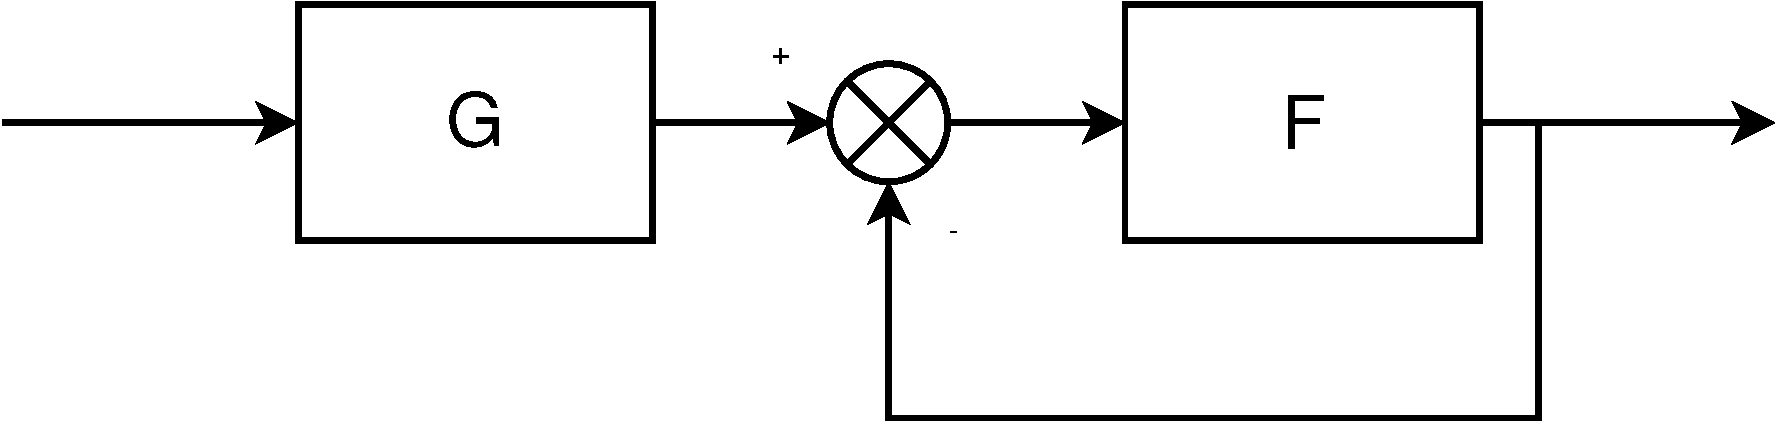
\includegraphics[width=8cm,
  keepaspectratio]{figuras/sistema1}



  \caption{\label{cap:DBloques}Diagrama de bloques del sistema
    ejemplo}
\end{figure}


Primero construiremos el bloque de la derecha, el más cercano a la
salida. Su función de transferencia es:
$DCHA(s)=\frac{10}{s^{2}(s+3)}$ de modo que empezaremos definiendo su
bloque básico:
\begin{verbatim}
>> DCHA=zp([],[0,0,-3],10,TSAM=0,'DCHAIN','DCHAOUT');
\end{verbatim} El paso siguiente es duplicar su salida 
\begin{verbatim}
>> DCHAdup=sysdup(DCHA,[],'DCHAIN');
DCHAdup =
{
  a =

    -3   1   0
     0   0   1
     0   0   0

  b =

    0  0
    0  0
    1  1

  c =

    10   0   0

  d =

    0  0

  inname =

  {
    [1,1] = DCHAIN
    [1,2] = DCHAIN(dup)
  }

  n = 3
  nz = 0
  outname =

  {
    [1,1] = DCHAOUT
  }

  stname =

  {
    [1,1] = x_1
    [1,2] = x_2
    [1,3] = x_3
  }

  sys =

    2  0  0  1

  tsam = 0
  yd = 0
}

\end{verbatim}
Como vemos ha aparecido una nueva entrada llamada
\texttt{DCHAIN(dup)}, copia de \texttt{DCHAIN}. Ahora ya podemos crear
la recirculación del primer estadio no sin antes cambiar el signo de
la nueva puerta de salida:
\begin{verbatim}
>> DCHAdup=sysscale(DCHAdup,[],diag([1,-1]));
\end{verbatim} 
Este es un modo abrevidado de utilizar la función \texttt{syscale},
consultando la ayuda aprenderemos a utilizarla de un modo más
intuitivo.  Ahora conectamos la señal a la salida con la nueva puerta
de entrada y finalmente simplificamos el sistema par que tenga una
única entrada.  Como paso final comprobaremos que el resultado es
realmente el deseado escribiendo la función de transferencia del
sistema.

\begin{verbatim}
>> DCHAend=sysconnect(DCHAdup,'DCHAOUT','DCHAIN(dup)');
>> DCHAend=sysprune(DCHAend,'DCHAOUT','DCHAIN');
>> sysout(DCHAend,'tf')
Input(s)
      1: DCHAIN

Output(s):
     1: DCHAOUT

transfer function form:
10
----------------------------------
1*s^3 + 3*s^2 + 1.554e-15*s^1 + 10
\end{verbatim} 

La definición del bloque de la izquierda es la única limitación del
OCTS. No puede definir bloques cuyo número de ceros sea mayor a su
número de polos. Esto es debido a la forma que tiene de hacer los
cálculos internos para crear la estructura de datos. Para seguir con
el ejemplo tendremos que romper la estructura de datos creada por el
primer bloque con recirculación, multiplicarla por el polinomio del
bloque de la izquierda y finalmente crear la última recirculación.
Esto no significa ningún problema porque podemos pasar de la
representación como estructura a función de transferencia sólo con
aplicar la función \texttt{sys2tf}
\begin{verbatim}
>> [num,den]=sys2tf(DCHAend);
\end{verbatim} 
Para multiplicar el numerador de la función de transferencia por el
nuevo término utilizamos la función \texttt{conv} que ya vimos en la
sección dedicada al cálculo con polinomios.
\begin{verbatim}
>> num=conv([1,2],num);
\end{verbatim} 
El paso siguiente es reconvertir la función de transferencia en el
tipo estructura.
\begin{verbatim}
>> TOTAL=tf(num,den,TSAM=0,'IN','OUT');
>> sysout(TOTAL,'tf')
Input(s)
      1: IN

Output(s):
     1: OUT

transfer function form:
10*s^1 + 20
----------------------------------
1*s^3 + 3*s^2 + 1.554e-15*s^1 + 10
\end{verbatim}


\subsection{Análisis en frecuencia}

\label{sec:analisis}

De nada servirían todas las funciones de construcción de bloques si
luego no podemos analizar el comportamiento de nuestro sistema. Esta
parte del toolkit es sin duda su punto fuerte.

Una de las pocas cosas que debemos tener en cuenta es que el sistema
que se estáresolviendo cuando se hace el análisis en frecuencias no
es el original sino el de la figura \ref{cap:DBloques2}:

%
\begin{figure}

 \centering{} 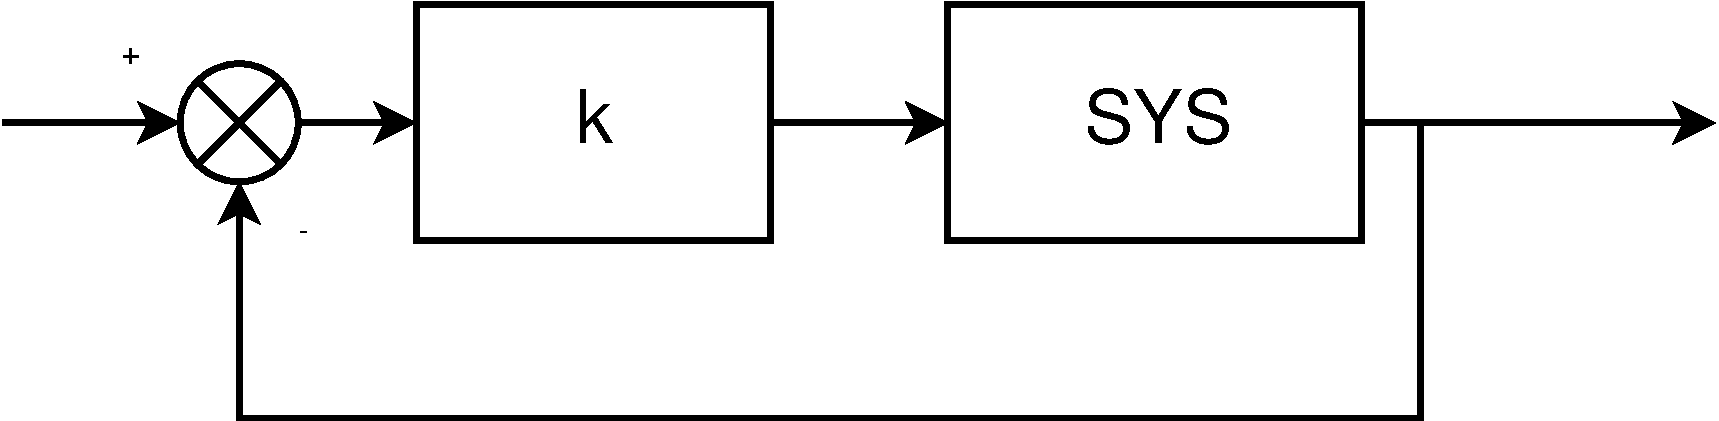
\includegraphics[width=8cm, keepaspectratio]{figuras/sistema2}


\caption{\label{cap:DBloques2}Diagrama de bloques resuelto}
\end{figure}


\begin{description}
\item [bode\index{bode}]Hace el análisis bode del sistema. En el caso
que no se soliciten argumentos de salida se dibuja el diagrama bode 
\item [nyquist\index{nyquist}]Hace el análisis nyquist de sistema. 
\item [nichols\index{nichols}]Hace en análisis nichols del sistema. 
\end{description}

\subsubsection{Ejemplo de análisis en frecuencia}

\label{sec:ejercicioanalisis} Aprovechando que ya hemos creado un
sistema en la sesión para hacer el diagrama de Nyquist basta con:
\begin{verbatim}
>> nyquist(TOTAL)
\end{verbatim} Lo que genera la figura (\ref{fig:nyquist}). %
\begin{figure}
 \centering
    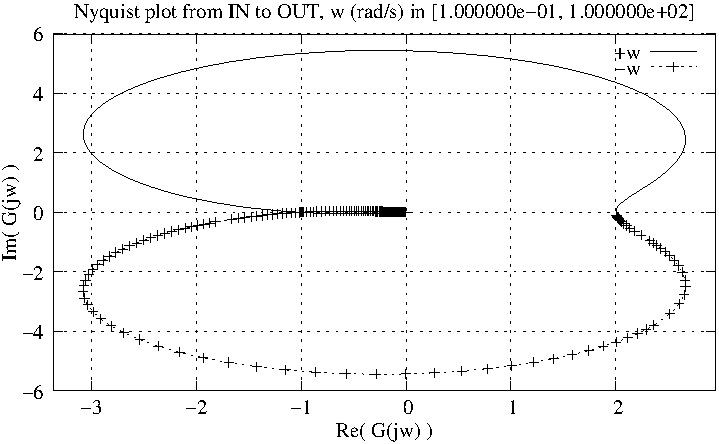
\includegraphics[width=12cm, keepaspectratio]{figuras/nyquist}


\caption{\label{fig:nyquist}Diagrama de Nyquist del sistema}
\end{figure}


Los diagramas de bode son igualmente sencillos de conseguir (figura
\ref{cap:bode}): 
\begin{verbatim}
>> bode(TOTAL)
\end{verbatim}%
\begin{figure}
 \centering
    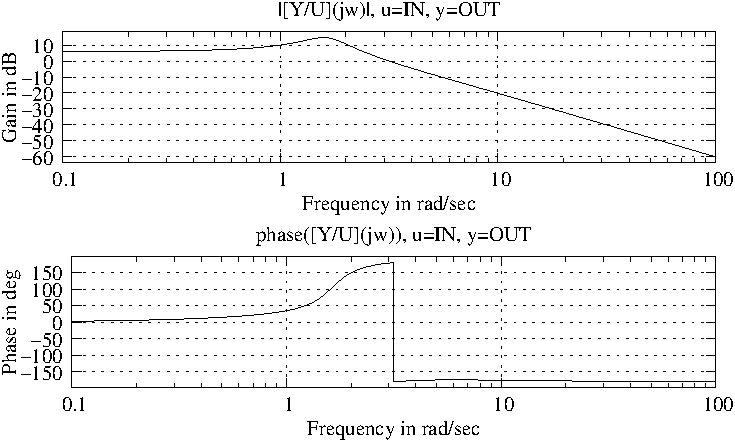
\includegraphics[width=12cm, keepaspectratio]{figuras/bode}

\caption{\label{cap:bode}Gráfica bode del sistema}
\end{figure}



\section{Resolución de EDPs, formulación diferencial.}
